\chapter{Bedrijf}
\label{ch:bedrijf}
Dit hoofdstuk biedt informatie over het bedrijf waarbij het onderzoek is uitgevoerd. Hiernaast geeft het inzicht in welke afdeling van het bedrijf het onderzoek gedaan is. 

\section{\&ranj}
\&ranj is een internationaal bedrijf dat sinds 1999 serious game oplossingen realiseert. Dit zijn spellen waarbij de speler spelenderwijs getraind wordt. Een voorbeeld hiervan is de serious game ‘Mission Zhobia – Winning the Peace’\footnote{\url{https://www.missionzhobia.org/}}. In deze game wordt de speler getraind in peace building. Het bedrijf heeft te maken met klanten in diverse vakgebieden. Hierdoor is het domein van de onderwerpen erg breed.

\&ranj wilt mensen helpen ontwikkelen op een effectieve en efficiënte manier. Met behulp van ‘serious games’ wilt het bedrijf voor de gebruiker een ervaring creëren waarin hij of zij kennis opdoet om in het echte leven uitdagingen aan te gaan en leert problemen te tackelen. Volgens \&ranj is de beste manier van leren het leren door te doen.

\section{Visie}
Met serious games past \&ranj op spelenderwijze gedragsverandering toe, om zo een betere toekomst te bouwen. De visie van \&ranj luidt:

\begin{quote} 
    \centering
    \large
    \textit{
        “Together we build a brighter future”
    }
\end{quote}

\section{Afdelingen}
Het bedrijf specialiseert zich in drie verschillende richtingen met ieder zijn eigen specialiteit. Deze richtingen kunnen omschreven worden met verschillende keywords.
\begin{itemize}
    \item Gamification; gefocust op: “consultancy”, “leuk maken van minder leuke taken/ werk”, “fysiek”.
    \item Playground; gefocust op: “experimentatie” en “ervaringen”.
    \item Corporate Learning; gefocust op: “soft skills”, “volwassen organisaties”, “bewezen oplossingen” en “efficiëntie”.
\end{itemize}
Dit onderzoek vindt plaats in de 'corporate learning’ afdeling.

\section{Corporate learning}
De corporate learning afdeling van \&ranj realiseert oplossingen voor “volwassen” bedrijven die soft skills bij hun werknemers willen bevorderen. Bij deze afdeling ligt de nadruk op efficiëntie en het gebruikt van oplossingen waarvan het bedrijf weet dat ze werken. Meestal zijn deze oplossingen narrative games, spellen waarin op verhalende wijze kennis wordt overgebracht.

Het ontwikkelen van een narrative game is een grote compliceert proces. Dit onderzoek zal zich alleen focussen op de ontwikkelingsfase, omdat de editors een grote rol in spelen. In deze fase werkt het team samen om het product te realiseren.

\begin{wrapfigure}{r}{0.45\textwidth}
    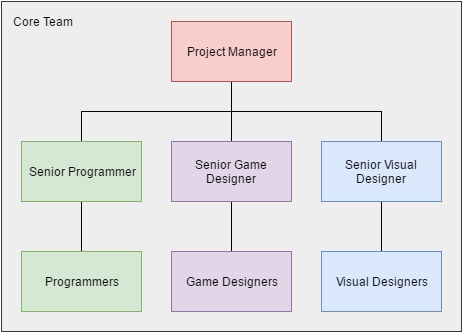
\includegraphics[width=0.43\textwidth]{CoreTeam}
    \caption{Anatomie van een core team bij \&ranj.}
    \label{fig:coreteam}
    \centering
\end{wrapfigure}

Een corporate learning development team bestaat uit de volgende disciplines:

\begin{description}
    \item[Programmeur] Is verantwoordelijk voor de technische implementatie van de game. Hiernaast biedt deze ondersteuning bij technische vraagstukken. 
    \item[Game designer] Is verantwoordelijk voor de mechanieken en het verhaal achter de game. Hij of zij probeert gedragsverandering toe te passen met de game als tool. Verder werken game designers nauw samen met de projectmanager om te zorgen dat de game aansluit bij de wensen van de klant.
    \item[Visual designer] Is verantwoordelijk voor de visuals binnen de game. Een visual designer wilt door middel van deze visuals meestal een gevoel bij de speler ontvlammen.
    \item[Projectmanager] Begeleid het ontwikkelproces en is regelmatig in contact met de klant. Hij of zij zorgt dat het project binnen het budget blijft en onderhandeld met de klant wanneer nodig. De projectmanager trekt aan de bel als het project niet aansluit bij de wensen van de klant en heeft veto op de keuzes binnen het project.    
\end{description}

Het kan zijn dat er meerdere programmeurs, game designers of visual designers aan een project werken. Als dit het geval is wordt er een senior als lead aangewezen. De lead begeleid de teamleden met dezelfde rol.

\subsection{Ontwikkelproces van narrative games}
Het ontwikkelen van een narrative game kan een ingewikkeld proces zijn dat veel tijd kan kosten. Dit ligt aan de complexiteit van het verhaal en eventuele achterliggende modellen. In het verhaal kan de speler keuzes maken waarbij elke keuze meestal tot een ander pad in het verhaal leidt.

Dit maakt het onmogelijk om het verhaal te definiëren in code of een bestaand dataformaat. Tenslotte wordt het handmatig vast leggen van het verhaal in een dataformaat zoals JSON of XML al gauw onoverzichtelijk. Dit zorgt voor een probleem in het ontwikkelproces.

Om dit probleem te tackelen en het ontwikkelproces efficiënter te laten verlopen heeft het bedrijf in 2008 het ontwikkelproces van narrative games gestandaardiseerd. Onder efficiënt verstaan we in dit geval het versnellen van het proces en het voorkomen van fouten in de game. 

Ter ondersteuning en standaardisatie van het ontwikkelproces zijn de story- en dialog editor gebouwd. Deze editors laten game designers zonder enige programmeerkennis verhalen en dialogen schrijven.

Om de efficiëntie van het ontwikkelproces van een narrative game verder te verhogen heeft het bedrijf een template opgezet voor het ontwikkelen van narrative games. Dit template noemen ze het narrative game template (NGT) en dient als een geteste basis voor narrative games. Het NGT verwerkt geëxporteerde data uit de story- en dialog editor en is het deel dat uiteindelijk de verschillende content types toont/ evalueert.
